\section[Reazioni Termonucleari]{Produzione di energia tramite reazioni termonucleari}\label{sec:reazioni-termonucleari}
Le \emph{reazioni termonucleari} sono la principale fonte di energia in una stella. La \emph{fusione} di elementi leggeri in elementi più pesanti produce non solo \emph{energia}, ma anche \emph{nuovi elementi}. Come nel caso dell'opacità i processi sono molto complessi e utilizzeremo solamente delle equazioni approssimate. Si faccia attenzione al fatto che i processi di fusione termonucleare coinvolgono solamente i \emph{nuclei} dell'atomo, perché le temperature sono così elevate ($T > \SI{e6}{K}$) che tutti gli atomi si possono considerare completamente ionizzati.

L'equazione di produzione di energia attraverso \emph{reazioni termonucleari} appare nella seguente maniera:
\begin{equation}\label{eq:reazioni-termonucleari}
    \epsilon = \epsilon(X, \rho, T) 
    \begin{cases} \epsilon_{PP} = \epsilon_1 \rho X^2 T_6^\alpha \quad \alpha \in [3.5 - 6] \\ 
    \epsilon_{CN} = \epsilon_2 \rho X X_{CN} T_6^\beta \quad \beta \in [13 - 20] \\ 
    \epsilon_{3\alpha} = \epsilon_3 \rho^2 Y^3 T_8^\gamma \quad \gamma \in [20 - 30] \\
    \end{cases}
\end{equation}
È dapprima necessario introdurre dei concetti di base sulla reazioni termonucleari.

\subsection{Ripasso di fisica nucleare}
\paragraph{Numero atomico e numero di massa}
Nel presente paragrafo si farà una veloce rassegna dei concetti di fisica nucleare utili per proseguire il discorso.

Ogni elemento chimico è univocamente identificato dal suo \emph{numero atomico} $Z$, corrispondente al numero di protoni nel nucleo. Il \emph{peso atomico} $A$ è il numero totale di nucleoni, ovvero la somma di protoni e neutroni. Gli \emph{isotopi} hanno stesso $Z$ ma diverso $A$.

\paragraph{Difetto di massa}
Nelle reazioni di fusione termonucleare, nuclei di elementi leggeri si fondono tra loro generando nuclei di elementi più pesanti ($Z$ più alto) ed energia. Pertanto, a causa della nota relazione massa-energia, la somma delle masse dei nuclei leggeri che fondono tra loro è maggiore della massa del nucleo più pesante che viene generato, e si può scrivere:
\begin{equation}\label{eq:difetto-massa}
    E = \Delta m \, c^2
\end{equation}
Guardando la carta dei nuclidi che rappresenta l'energia di legame per nucleone (fig.~\ref{fig:energia-legame}), possiamo stabilire che è grazie alle reazioni di fusione del nucleo delle stelle che sono stati prodotti tutti gli elementi più pesanti dell'elio ($Z=2$) fino al ferro ($Z=26$), come verrà riassunto successivamente.

\paragraph{Energia di legame}
All'interno del nucleo atomico, i nucleoni sono legati tra loro dalla \emph{forza forte}, la quale agisce su distanze estremamente piccole ($\sim \SI{e-12}{cm}$ -- $\SI{e-13}{cm}$). La massa totale del nucleo è sempre minore della somma di tutti i nucleoni che lo costituiscono. Questo si spiega attraverso il difetto di massa, eq.~\eqref{eq:difetto-massa}, e permette di definire l'\emph{energia di legame} come:
\begin{equation}\label{eq:energia-legame}
    E(Z,N) = \bigl[ Z m_p + N m_n - m(Z,n) \bigr] \, c^2
\end{equation}

con $Z$ il numero di protoni, $N$ il numero di neutroni, $m_p = \SI{1.672e-24}{g}$ la massa del protone, $m_n = \SI{1.675e-24}{g}$ la massa del neutrone e $m(Z,n)$ la massa del nucleo. Questo significa che quando si forma un nuovo nucleo stabile, una certa frazione di massa viene trasformata in energia secondo la~\eqref{eq:energia-legame}, ovvero, $E(Z,N)$ è l'energia che viene prodotta quando si forma un nuovo nucleo stabile, ovvero $E(Z,N)$ è l'energia che bisogna fornire ad un nucleo per spaccarlo nei singoli nucleoni che lo costituiscono.

\paragraph{Energia di legame per nucleone dei nuclidi stabili}

\begin{figure}
    \centering
    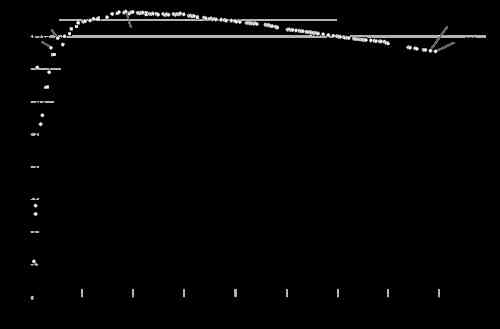
\includegraphics[width=0.7\textwidth]{immagini/energia-legame.jpg}
    \caption{Energia di legame media per nucleone. Si noti come \ce{^4He} sia particolarmente stabile, fino al ferro domina la fusione e dopo il ferro domina la fissione.}
    \label{fig:energia-legame}
\end{figure}

Consideriamo l'\emph{energia di legame media per nucleone}, plottata in fig.~\ref{fig:energia-legame}, e corrispondente, secondo la~\eqref{eq:energia-legame} a $E(Z,N) / A$. Dalla figura possiamo trarre alcune considerazioni generali:
\begin{itemize}
    \item ci sono configurazioni nucleari particolarmente stabili quali \ce{^4He}, \ce{^{12}C}, \ce{^{16}O} \dots
    \item a parte queste eccezioni, l’energia di legame media per nucleone, $E/A$, ha un andamento regolare. Aumenta rapidamente con il numero di nucleoni fino ad un valore dell’ordine degli $\SI{8}{Mev}$ per poi diminuire assai lentamente (\emph{proprietà di saturazione}).
    \item i nuclei più stabili sono il \ce{^{56}Fe} e il \ce{^{62}Ni}. Ciò significa che i nuclei pesanti alla sua destra possono raggiungere configurazioni più stabili ($B/A$ più elevato) diminuendo il numero di nucleoni $A$, ovvero frazionandosi in nuclei più piccoli. Mentre i nuclei leggeri alla sua sinistra possono raggiungere configurazioni più stabili ($B/A$ più elevato) aumentando $A$, ovvero aggregandosi in nuclei più grandi. Detto in altri termini ciò significa che le reazioni di fissione dei nuclei pesanti e quelle di fusione dei nuclei leggeri sono esoenergetiche ovvero producono energia qualora si sia in grado di innescarle.
    \item dal punto precedente consegue che le reazioni di \emph{fusione dei nuclei leggeri} e \emph{fissione dei nuclei pesanti} costituiscono la doppia opportunità offerta dalla fisica nucleare per la produzione di energia.
\end{itemize}

\paragraph{Barriera di potenziale ed effetto tunnel}
Da un punto di vista \emph{classico} la reazione di fusione avviene se due nuclei riescono ad avvicinarsi a meno della distanza $R_0$ necessaria per far entrare in gioco le interazioni forti, ovvero solo dopo aver superato la barriera di potenziale in fig.~\ref{fig:barriera-potenziale}

\begin{figure}
    \centering
    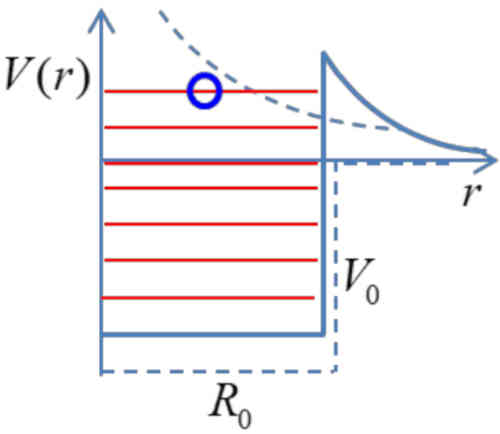
\includegraphics[width=0.3\textwidth]{immagini/barriera-potenziale.jpg}
    \caption{Barriera di potenziale. È data dalla sovrapposizione del potenziale attrattivo della forza forte, che agisce per $r < R_0$ e della forza repulsiva Coulombiana, che agisce per $r > R_0$ e vale $E_c = Z_1 Z_2 e^2 / r$.}
    \label{fig:barriera-potenziale}
\end{figure}

Facendo una stima molto rozza, possiamo trovare che la barriera di potenziale è circa $1000$ volte superiore all'energia termica media delle particelle, quindi, anche ad elevatissime temperature, è molto improbabile che le reazioni possano avvenire. Dal punto di vista quantistico questo si spiega con il così detto \emph{effetto tunnel}.

\paragraph{Pricnicpali catene di fusione termonucleare nelle stelle}
Di seguito sono elencate le principali catene di fusione nelle stelle, le quali saranno approfondite nei successivi paragrafi:
\begin{description}
    \item[Catena PP] Processo di bruciamento dell'idrogeno. È un processo di cattura protonica. Avviene per $T \simeq \SI{e7}{K}$.
    \item[Catena CNO] Processo di bruciamento dell'idrogeno. È un processo di cattura protonica. Avviene per $T \simeq \SI{1.8e7}{K}$.
    \item[Catena 3-alpha] Processo di bruciamento dell'elio. Avviene per temperature $T \simeq \SI{1.5e8}{K}$.
    \item[Cattura alpha] Il carbonio e materiali più pesanti catturano particelle $\alpha$ per produrre materiali più pesanti. Avviene per $T > \SI{5e8}{K}$.
\end{description}

\subsection{Catena protone--protone}\label{sec:catena-pp}
\paragraph{Catena PPI}
La catena \emph{protone--protone PPI} è rappresentata in fig.~\ref{fig:catena-pp1}. È una reazione di bruciamento dell'idrogeno e dà elio. Può essere scritta nella seguente maniera:
\reaction[re:pp1]{H^1 + H^1 -> H^2 + e^+ + $\nu$}
\reaction[re:pp2]{H^2 + H^1 -> He^3 + $\gamma$}
\reaction[re:pp3]{He^3 + He^3 -> He^4 + H^1 + H^1}
ovvero, in definitiva da \ce{4 H} ottengo \ce{1 He^4}, e siccome \ce{1 He^4} pesa meno di \ce{4 H}, dall'eq.~\eqref{eq:difetto-massa} possiamo stabilire che la reazione è \emph{esotermica}.

\begin{figure}
    \centering
    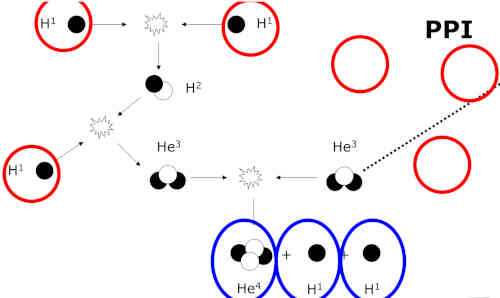
\includegraphics[width=0.5\textwidth]{immagini/catena-pp1.jpg}
    \caption{Catena protone-protone (PPI).}
    \label{fig:catena-pp1}
\end{figure}

Facciamo una stima dei contributi energetici. Il neutrino $\nu$ porta un contributo energetico \emph{negativo}, perché avendo una scarsa interazione con la materia tendono a sfuggire dalla struttura stellare. Senza aggiungere ulteriori specificazioni, si ricordi che, tenuti in considerazione tutti i contributi, l'energia totale prodotta dalla reazione PPI è:
\begin{equation}\label{eq:energia-pp1}
    E_\textup{PPI} = \SI{26.2}{MeV} = \SI{4.2e-5}{erg}
\end{equation}

Senza scendere troppo nei dettagli, evidenziamo che il \emph{tempo scala} della reazione~\ref{re:pp1} è $t_1 = \SI{1.4e9}{yr}$, il tempo scala della reazione~\ref{re:pp2} è $t_2 = \SI{6}{s}$ e il tempo scala della reazione~\ref{re:pp3} è $t_3 = \SI{e6}{yr}$. Dunque, ricordando che la \emph{probabilità} che avvenga la reazione è proporzionale all'inverso del tempo scala, possiamo stabilire che la prima reazione è molto improbabile che avvenga, mentre la seconda è molto probabile. In particolare, concentriamoci sulla prima reazione (~\ref{re:pp1}). Essa trasforma due protoni liberi (\ce{H}) in un nucleo costituito da un protone e un neutrone (\ce{H^2}). Significa che uno dei due protoni si è trasformato in neutrone. Quindi, affinché la reazione possa avvenire, è necessario che ci sia un \emph{decadimento $\beta$}, espresso dalla seguente equazione:
\reaction[re:decadimento-beta+]{p^+ -> n + e^+ + $\nu$}
Tuttavia, il decadimento $\beta^+$ per un protone libero è essenzialmente impossibile, poiché la massa del protone è minore della massa del neutrone (eq.~\eqref{eq:difetto-massa}). Nonostante ciò, nel nucleo delle stelle tale reazione può avvenire poiché ci sono tantissimi protoni, dunque anche se la probabilità è bassissima, questa è compensata dall'elevato numero. 

D'altra parte, il \emph{decadimento $\beta^-$}, secondo il quale un neutrone decade in protone, è un processo spontaneo, in quanto il suo tempo scala è dell'ordine di $\SI{800}{s}$ e tende ad eliminare tutti i neutroni liberi:
\reaction[re:decadimento-beta-]{n -> p^+ + e^- + $\nu$}
Tuttavia negli interni stellari possono comunque esserci neutroni liberi, i quali contribuiscono alla formazione di elementi più pesanti, come vedremo successivamente.

\paragraph{Catena PPII e PPIII}
Consideriamo le reazioni~\ref{re:pp1} e~\ref{re:pp2}. Con una probabilità $P_1 = 69 \%$ può avvenire, successivamente, la reazione~\ref{re:pp3}, dando origine alla catena PPI. Tuttavia, non si tratta dell'unica possibilità. Infatti, con una probabilità residua del $31\%$, può avvenire la seguente reazione:
\reaction[re:ppsecondaria]{He^3 + He^4 -> Be^7 + $\gamma$}
Se inizialmente prevale la PPI, dopo un po' che questa è attiva l'ambiente si popola di \ce{He^2} e può facilmente avvenire la~\ref{re:ppsecondaria}, che produce energia. Se è attivo tale canale, quasi sempre la catena prosegue con la PPII (fig.~\ref{fig:catena-pp2}), con una probabilità $P_2=99.7\%$, nella seguente maniera:
\reaction[re:ppII1]{Be^7 + e^- -> Li^7 + $\nu$}
\reaction[re:ppII2]{Li^7 + H^1 -> Be^8}
\reaction[re:ppII3]{Be^8 -> 2 He^4 + $\gamma$} 
In particolare, nella~\ref{re:ppII3} il \ce{Be^8} è instabile e si spacca in due nuclei di \ce{He^4}, producendo energia, a causa della sua elevata stabilità, come si nota anche in fig.~\ref{fig:energia-legame}.

\begin{figure}
    \centering
    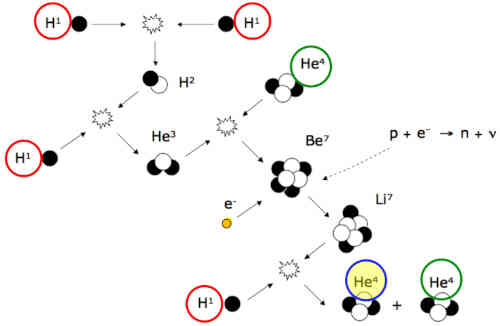
\includegraphics[width=0.5\textwidth]{immagini/catena-pp2.jpg}
    \caption{Catena protone-protone (PPII).}
    \label{fig:catena-pp2}
\end{figure}

Con una probabilità residua di $P_3 = 0.3\%$, la \ref{re:ppsecondaria} può proseguire con una catena PPIII (fig.~\ref{fig:catena-pp3}), nella seguente maniera:
\reaction[re:ppIII1]{Be^7 + H^1 -> B^8 + $\gamma$}
\reaction[re:PPIII2]{B^8 -> Be^8 + e^+ + $\gamma$}
\reaction[re:PPIII3]{Be^8 -> 2 He^4 + $\gamma$}

\begin{figure}
    \centering
    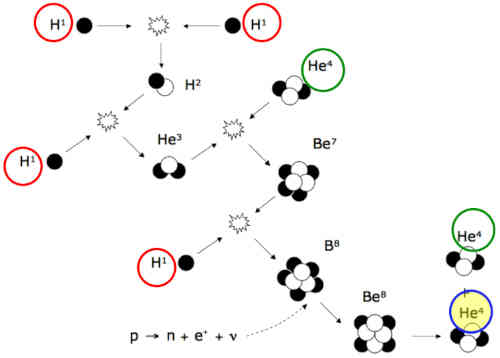
\includegraphics[width=0.5\textwidth]{immagini/catena-pp3.jpg}
    \caption{Catena protone-protone (PPIII).}
    \label{fig:catena-pp3}
\end{figure}

In tutti i casi, tuttavia, brucio \ce{4 H} per generare \ce{1 He^4}, producendo un'energia di $\sim \SI{20}{Mev}$. In particolare si ha: $E_\textup{PPI} = \SI{26.2}{Mev}$, $E_\textup{PPII} = \SI{25.7}{Mev}$ e $E_\textup{PPIII} = \SI{19.3}{Mev}$. 

\subsection{Catena CNO}\label{sec:catena-cno}
Un'altra possibile catena di bruciamento dell'idrogeno, è la così detta \emph{catena CNO}, detta anche \emph{CN--NO}. A differenza della precedente (par.~\ref{sec:catena-pp}), richiede la presenza di carbonio, azoto e ossigeno. Si noti che questi ultimi elementi \emph{non} sono prodotti dalla catena di reazione, ma devono essere già presenti nel gas, agendo come catalizzatori. Il ciclo principale della catena è raffigurato in fig.~\ref{fig:catena-cno} e può essere sintetizzato dalle seguenti reazioni:
\reaction[re:cno1]{C^{12} + H^1 -> N^{13} + $\gamma$}
\reaction[re:cno2]{N^{13} -> C^{13} + e^+ + $\nu$}
\reaction[re:cno3]{C^{13} + H^1 -> N^{14} + $\gamma$}
\reaction[re:cno4]{N^{14} + H^1 -> O^{15} + $\gamma$}
\reaction[re:cno5]{O^{15} -> N^{15} + e^+ + $\nu$}
\reaction[re:cno6]{M^{15} + H^1 -> C^{12} + He^4}

\begin{figure}
    \centering
    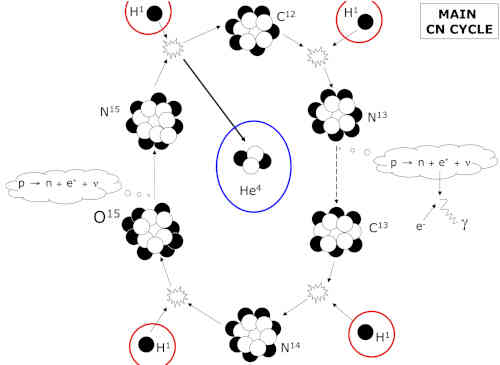
\includegraphics[width=0.5\textwidth]{immagini/catena-cno.jpg}
    \caption{Catena CN--NO. Partendo da \ce{C^{12}}, la parte sinistra rappresenta il ramo rapido, mentre la parte destra, che parte da \ce{N^{14}} rappresenta il ramo lento.}
    \label{fig:catena-cno}
\end{figure}

In totale il ciclo utilizza \ce{4 H} e genera \ce{1 He^4}. Facendo un computo delle energie, si ha:
\begin{equation}\label{eq:energia-cno}
E_\textup{CNO} = \SI{25}{MeV} \simeq \SI{2e-5}{erg}
\end{equation}
dello stesso ordine di grandezza dell'energia delle catene PP~\eqref{eq:energia-pp1}. Senza approfondire tutti i tempi scala, si sottolinea che quello della reazione~\ref{re:cno4} è dell'ordine di $\SI{3.2e8}{yr}$, dividendo la catena in un ramo rapido (da~\ref{re:cno1} a~\ref{re:cno4}) e un ramo lento (da~\ref{re:cno4} a~\ref{re:cno6} e nuovamente~\ref{re:cno1}). Quindi, nelle stelle in cui avviene il ciclo CNO mi aspetto che, se il materiale processato va verso la superficie per convezione, deve esserci una variazione delle abbondanze chimiche. In particolare, mi aspetto che l'abbondanza del carbonio diminuisca e quella dell'azoto e dell'ossigeno aumentino. Infine, sottolineiamo che questa reazione è un prototipo di reazione di cattura protonica.

\subsection{Il problema dell'elio}
Dopo aver visto alcune catene di bruciamento dell'idrogeno, soffermiamoci sul \emph{problema dell'elio}. Esso consiste nel fatto che l'abbondanza di \ce{He} che si misura nell'universo è troppo alta per essere spiegata solo in base al bruciamento dell'idrogeno negli interni stellari.

Considerato che nell'universo si misura un'abbondanza di \ce{He} pari a
\begin{equation}\label{eq:abbondanza-elio-misurata}
    Y \sim 0.24 - 0.28
\end{equation}

Stimiamo, quindi, quanto \ce{He} può essere stato prodotto dalle stella da quando si è formato l'universo, ovvero in un tempo di Hubble ($t_H \sim \SI{13}{Gyr}$), facendo un conto per la Via Lattea, della quale conosciamo la massa $M_G$ e la luminosità $L_G$
\[
M_G \sim \SI{e12}{\solarmass} \qquad M_G \sim \SI{e11}{\solarluminosity}
\]
e supponendo che tutta la luminosità della Galassia venga dal bruciamento di idrogeno in elio e che sia rimasta sempre costante. In questo modo dovrei sovrastimare il valore reale. Ricordando che la luminosità è l'energia prodotta per unità di tempo (par.~\ref{sec:luminosità}), per $L_G$, in un tempo $t_H$ si trova un'energia:
\[
E_\textup{tot} \simeq L_G t_H \sim \SI{1.6e62}{erg}
\]
che rappresenta l'energia totale prodotta dal bruciamento di \ce{H} in \ce{He} da quando si è formata la Galassia. Considerato che l'energia di legame di un nucleo di \ce{He} è
\[
E_\textup{b, He} \sim \SI{4.5e-5}{erg}
\]
e che può essere pensata come l'energia prodotta dal bruciamento di 4 nuclei di \ce{H} in un nucleo di \ce{He}, possiamo trovare il numero di atomi di \ce{He^4} che si sono formati dalla formazione della Galassia:
\[
N_\textup{He} = \frac{E_\textup{tot}}{E_\textup{b, He}} \simeq \SI{3.5e66}{}
\]
Possiamo pensare questo numero come il numero di reazioni di bruciamento di idrogeno che sono avvenute. Ora, dalla massa di un atomo di elio, $m_\textup{He} \sim \SI{6.64e-24}{g}$, possiamo ricavare la massa totale di \ce{He} prodotta in un tempo di Hubble:
\[
M_\textup{He} = N_\textup{He} m_\textup{He} \sim \SI{2.4e43}{g}
\]
Infine, usando $M_G$ possiamo trovare la frazione in massa di elio prodotta dalle Via Lattea da quando l'universo si è formato:
\begin{equation}\label{eq:abbondanza-elio-stimata}
Y = \frac{M_\textup{He}}{M_G} \sim 0.01
\end{equation}
Confrontando la~\eqref{eq:abbondanza-elio-misurata} con la~\eqref{eq:abbondanza-elio-stimata}, notiamo come l'abbondanza di elio misurata sia circa 20 volte maggiore di quella stimata. Questo significa che una frazione rilevante di \ce{He} deve essere stata prodotta da un altro processo, molto più efficiente e primordiale: si tratta del \emph{Big Bang}. Infatti, un punto rilevante che esso riesce a spiegare è la formazione di \emph{deuterio} (\ce{H^2}), processo molto difficile nelle stelle a causa della carenza di neutroni liberi, che decadono spontaneamente in protoni per il decadimento $\beta^-$ (\ref{re:decadimento-beta-}). Tuttavia, nei primi minuti successivi al Big Banda, c'erano molti neutroni liberi disponibili, e dunque la seguente catena di reazioni spiega la formazione di una grande quantità di elio subito dopo il Big Bang:
\reaction[re:bb1]{n + p -> H^2 + $\gamma$}
\reaction[re:bb2]{H^2 + H^2 -> He^3 + n}
\reaction[re:bb3]{He^3 + n -> H^3 + p}
\reaction[re:bb4]{H^2 + H^3 -> He^4 + n}
Tale \emph{nucleosintesi primordiale} si è fermata all'elio e non ha prodotto elementi più pesanti, poiché le reazioni successive di cattura neutronica o protonica avrebbero prodotto elementi instabili. In definitiva, riteniamo che gran parte dell'elio sia stato prodotto durante il Big Bang, mentre gli elementi più pesanti siano prodotti negli interni stellari.
 
\subsection{Catena 3-alpha}
La \emph{catena 3-$\alpha$} è una catena di bruciamento dell'elio in carbonio. Si ricordi che una particella $\alpha$ non è altro che un nucleo di elio. Vediamo quando tale catena si innesca.

Quando il nucleo stellare è costituito quasi interamente da elio, le reazioni di bruciamento dell'idrogeno cessano e la struttura va fuori dall'equilibrio idrostatico. In questa situazione prevale la forza gravitazionale che fa contrarre il nucleo, provocando un conseguente aumento della temperatura. Quando le temperature raggiungono $T \sim \SI{1.5e8}{K}$, può avvenire la reazione di fusione termonucleare di \ce{He}. Le due reazioni salienti della catena 3-$\alpha$ sono le seguenti:
\reaction[re:3alpha1]{He^4 + He^4 <--> Be^8}
\reaction[re:3alpha2]{Be^8 + He^4 -> C^12 + $\gamma$}
Come si può notare, la reazione~\ref{re:3alpha1} è reversibile, e in particolare, a causa dell'elevata instabilità di \ce{Be^8}, appena questo si forma, in un tempo molto breve tende a spaccarsi nuovamente in \ce{2 He^4}. Tuttavia, in questo caso l'abbondanza di \ce{He} è così elevata che \ce{Be^8}, prima di decadere, si fonde con un altro \ce{He^4}, secondo la reazione~\ref{re:3alpha2}.

In definitiva \ce{2 He^4} vengono trasformati in un \ce{C^12}. Facendo un computo dell'energia si trova:
\begin{equation}\label{eq:energia-3alpha}
    E_{3\alpha} = \SI{7.3}{MeV} \simeq \SI{1.2e-5}{erg}
\end{equation}
e possiamo notare che viene prodotta molta meno energia dei processi di bruciamento dell'idrogeno,~\eqref{eq:energia-pp1} e~\eqref{eq:energia-cno}. In particolare, l'energia per unità di massa prodotta dal bruciamento dell'elio è $\sim 10\%$ di quella prodotta dal bruciamento dell'idrogeno. Questo ha un impatto sui \emph{tempi di evoluzione stellare}: la fase in cui viene bruciato idrogeno nel nucleo, detta \emph{sequenza principale} è molto più lunga della fase in cui viene bruciato elio nel nucleo, detta \emph{red clump} o \emph{horizontal branch}.

A questo punto, se la struttura è termoregolata (gas non degenere), esaurito l'elio, possono continuare processi di bruciamento di materiali sempre più pesanti, fino al silicio, che genera ferro. Infatti, dopo il ferro (fig.~\ref{fig:energia-legame}) i processi di fusione sono endotermici. Non ci soffermeremo sui dettagli di tali reazioni, tuttavia vogliamo richiamare l'attenzione sul fatto che durante tutte queste reazioni vengono prodotte tante particelle $\alpha$. Che fine fanno?

\subsection{Processi di cattura alpha}\label{sec:cattura-alpha}
Le particelle $\alpha$ possono essere catturate da particelle più pesanti generando elementi pesanti attraverso reazioni che necessitano di temperature più basse della fusione. Gli elementi prodotti da queste reazioni sono detti \emph{elementi-$\alpha$} e sono sostanzialmente tutti gli elementi dal carbonio al silicio. In generale, è più conveniente per un atomo pesante catturare una particella $\alpha$ che fondersi con essa, perché la temperatura di innesco è più bassa. Ovviamente, posso arrivare fino al ferro. E per gli elementi più pesanti?

\subsection{Processi di cattura neutronica}
Attraverso processi di \emph{cattura neutronica} si spiega la presenza di elementi più pesanti del ferro. Essi consistono nella cattura di un neutrone da parte di un elemento, il quale rimane lo stesso elemento chimico ($Z$ non varia), ma diventa un suo isotopo (il numero di massa $A$ aumenta di $1$). Tale isotopo spesso è instabile e decade in un elemento che ha un numero atomico maggiore. Si può riassumere nella seguente reazione:
\reaction[re:cattura-neutronica]{^A_ZX + n -> ^{A+1}_ZX -> ^{A+1}_{Z+1}X + e^- + $\Bar{\nu}$}
La catena può proseguire in questo moto, tuttavia non scendiamo nei dettagli. In generale, le catture elettroniche si dividono in catture \emph{lente}, che producono \emph{elementi s}, e catture \emph{rapide}, che producono \emph{elementi r}. Per capire in quale dei due casi si è, si compara il tempo di decadimento dell'isotopo con il tempo di acquisizione del neutrone. 

Affinché le reazioni di cattura neutronica possano avvenire, è necessario che ci siano neutroni liberi che possano essere catturati, tuttavia, per il decadimento $\beta^-$ (\ref{re:decadimento-beta-}), il quale è molto veloce e probabile, un neutrone tende a decadere in protone.  Le principali sorgenti di neutroni per i processi s sono i processi $\alpha$ (par.~\ref{sec:cattura-alpha}), i quali avvengono nel \emph{ramo asintotico delle giganti}, come vedremo in seguito. Per i processi r, invece, la fonte principale di neutroni liberi è la fotodisintegrazione del ferro, che avviene a temperature alte durante l'esplosione di una supernova di tipo II, di cui parleremo successivamente. 

\subsection{Tasso di produzione di energia}
I processi visti finora, riassunti in tab.~\ref{tab:processi-produzione-energia} e i cui prodotti sono raffigurati in fig.~\ref{fig:processi-produzione-energia}, rappresentano la fonte principale di energia in una stella. Ci proponiamo ora di calcolare il \emph{tasso di produzione di energia} $\epsilon$ per una stella, ovvero l'energia prodotta per unità di massa e unità di tempo. 

\begin{figure}
    \centering
    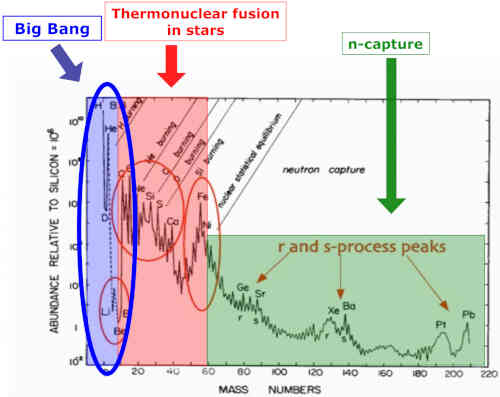
\includegraphics[width=0.5\textwidth]{immagini/processi-produzione-energia.jpg}
    \caption{Abbondanze degli elementi divise per i processi che li hanno generati in maniera preponderante.}
    \label{fig:processi-produzione-energia}
\end{figure}

\begin{table}
\caption{Principali reazioni nucleari.}
\label{tab:processi-produzione-energia}
\centering
\begin{tabular}{lll}
\toprule
Processo & Temperatura ($\si{K}$) & Tempo scala  ($\si{yr}$)\\
\midrule
Elementi leggeri & $\sim \SI{e6}{}$ & $\sim \SI{e5}{}$ \\
Catena PP & $\sim \SI{e7}{}$ & $\sim \SI{e10}{}$ \\
Catena CNO & $\sim \SI{e7}{}$ & $ \SI{e9}{}$\\
Catena 3--$\alpha$ & $> \SI{e8}{}$ & $\SI{e7}{}$ \\
Bruciamento carbonio & $\sim \SI{e9}{}$ & $\SI{e5}{}$ \\
Bruciamento Ossigeno & $> \SI{e9}{}$ & $\SI{e5}{}$ \\
Processo s & $> \SI{e8}{}$ & $\SI{e3}{}$--$\SI{e7}{}$ \\
Processo r & $> \SI{e10}{}$ & $\SI{10}{s}$--$\SI{100}{s}$ \\
\bottomrule
\end{tabular}
\end{table}

Essa può essere stimata così:
\begin{equation}
    \epsilon = \sum_{i=1}^{N_r} E_r \dfrac{N_r}{\si{g.s}} = \sum_{i=1}^{N_r} E_r \dfrac{N_r}{\si{cm^3.s}} \dfrac{\si{cm^3}}{\si{g}}
\end{equation}
dove con $i \in [N_r]$ si sta sommando sulle varie reazioni della catena in considerazione, $E_r$ è l'energia prodotta da ciascuna reazione, $N_r/\si{cm^3.s}$ è il numero di reazioni per unità di volume e di tempo e $\si{cm^3} / \si{g}$ rappresenta l'inverso della densità della materia stellare. Essa dipende da:
\begin{itemize}
    \item Carburante disponibile
    \item Temperatura (le reazioni si innescano dopo una certa soglia)
    \item Densità
\end{itemize}

In un modello stellare si esprime $\epsilon$ in maniera approssimata, in base alle proprietà macroscopica della struttura. In particolare possiamo scrivere:
\begin{subequations}
\label{eq:energia-reazioni-termonucleari}
\begin{align}
\epsilon_\textup{PP} &= \epsilon_1 \rho X^2 {T_6}^{\nu_\textup{PP}} \qquad \qquad \nu_\textup{PP} \in [3.5 - 6] \label{eq:energia-PP}\\
\epsilon_\textup{CN} &= \epsilon_2 \rho X X_\textup{CN} {T_6}^{\nu_\textup{CN}} \qquad \nu_\textup{CN} \in [13 - 20] \label{eq:energia-CN}\\
\epsilon_{3\alpha} &= \epsilon_3 \rho^2 Y^3 {T_8}^{\nu_{3\alpha}} \qquad \qquad \nu_{3 \alpha} \in [20 - 30] \label{eq:energia-3A}
\end{align}
\end{subequations}
dove $T_6$ significa che la temperatura è espressa in unità di $\SI{e6}{K}$, mentre $T_8$ significa che la temperatura è espressa in unità di $\SI{e8}{K}$. $X$ è l'abbondanza dell'idrogeno, $Y$ l'abbondanza dell'elio e $X_\textup{CN}$ l'abbondanza di carbonio e azoto. Si noti la mostruosa dipendenza dalla temperatura delle~\eqref{eq:energia-reazioni-termonucleari}, il che evidenzia che reazioni termonucleari stabili possono avvenire solamente in ambienti termonucleari, ovvero in cui il gas può essere considerato perfetto. Infatti, in ambienti degeneri, in cui la pressione non dipende dalla temperatura, siccome piccole variazioni di energia producono una variazione enorme della creazione di energia, la struttura può esplodere. Come si può notare, queste sono le espressioni che compaiono nell'equazione~\eqref{eq:reazioni-termonucleari}. 

\section{Riassunto sul modello stellare.}
Con le 7 equazioni presentate nel par.~\ref{sec:modelli-stellari} abbiamo un sistema di 7 equazioni in 7 incognite per descrivere la struttura di una stella. In particolare, le incognite sono:
\begin{itemize}
    \item La pressione $P$
    \item La massa $M$
    \item La densità $\rho$
    \item La luminosità $L$
    \item L'opacitk $\kappa$
    \item Il tasso di produzione di energia $\epsilon$
\end{itemize}
Queste equazioni descrivono l'interno stellare di una stella , dandomi in output la sua \emph{luminosità}. L'altro parametro di cui ho bisogno è la \emph{temperatura superficiale} della stella. Per ottenerla ho bisogno di un modello della sua atmosfera.